\documentclass[14pt]{extbook}
\usepackage{multicol, enumerate, enumitem, hyperref, color, soul, setspace, parskip, fancyhdr} %General Packages
\usepackage{amssymb, amsthm, amsmath, bbm, latexsym, units, mathtools} %Math Packages
\everymath{\displaystyle} %All math in Display Style
% Packages with additional options
\usepackage[headsep=0.5cm,headheight=12pt, left=1 in,right= 1 in,top= 1 in,bottom= 1 in]{geometry}
\usepackage[usenames,dvipsnames]{xcolor}
\usepackage{dashrule}  % Package to use the command below to create lines between items
\newcommand{\litem}[1]{\item#1\hspace*{-1cm}\rule{\textwidth}{0.4pt}}
\pagestyle{fancy}
\lhead{Makeup Progress Quiz -1}
\chead{}
\rhead{Version C}
\lfoot{7547-2949}
\cfoot{}
\rfoot{Fall 2020}
\begin{document}

\begin{enumerate}
\litem{
Choose the graph of the equation below.\[ f(x) = \sqrt{x - 8} + 7 \]\begin{enumerate}[label=\Alph*.]
\begin{multicols}{2}\item 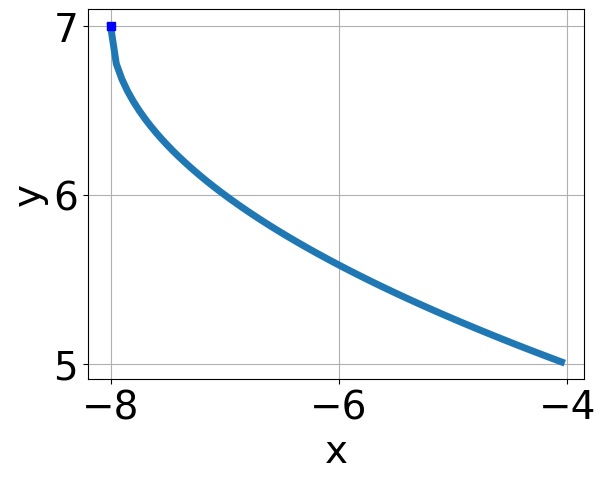
\includegraphics[width = 0.3\textwidth]{../Figures/radicalEquationToGraphCopyAC.png}\item 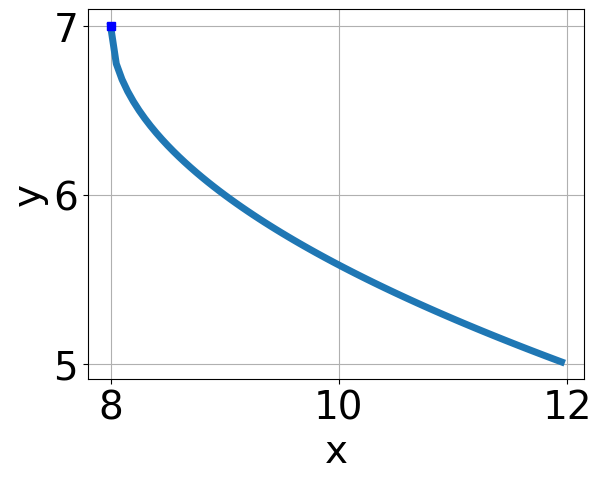
\includegraphics[width = 0.3\textwidth]{../Figures/radicalEquationToGraphCopyBC.png}\item 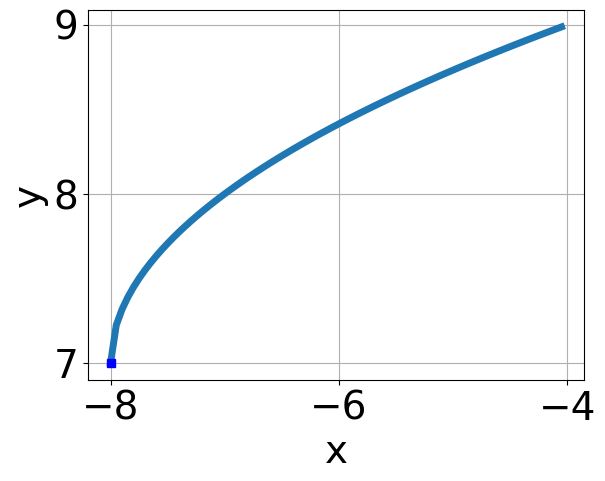
\includegraphics[width = 0.3\textwidth]{../Figures/radicalEquationToGraphCopyCC.png}\item 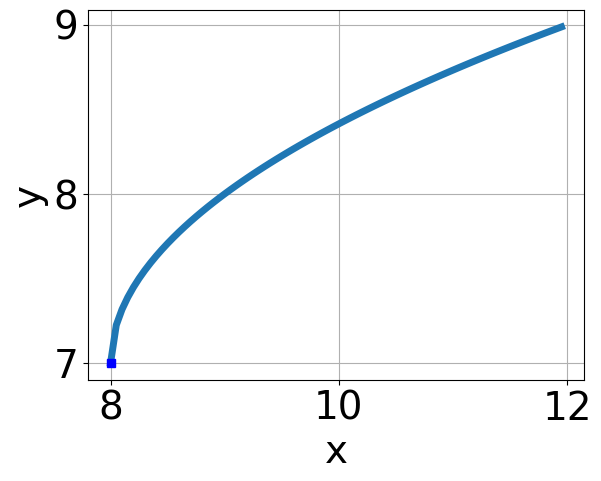
\includegraphics[width = 0.3\textwidth]{../Figures/radicalEquationToGraphCopyDC.png}\end{multicols}\item None of the above.
\end{enumerate} }
\litem{
Choose the graph of the equation below.\[ f(x) = - \sqrt[3]{x + 8} - 5 \]\begin{enumerate}[label=\Alph*.]
\begin{multicols}{2}\item 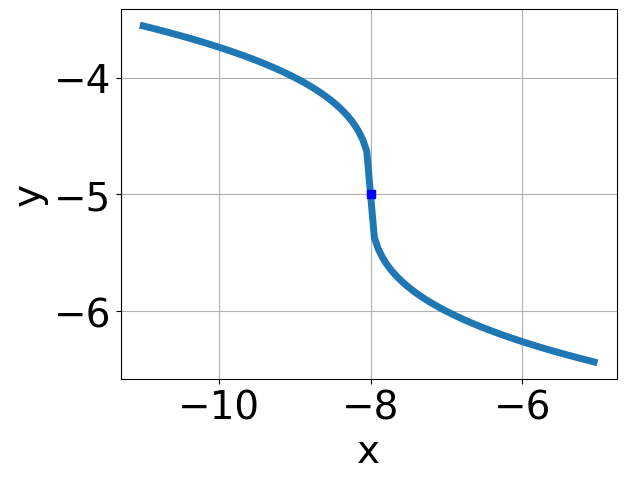
\includegraphics[width = 0.3\textwidth]{../Figures/radicalEquationToGraphAC.png}\item 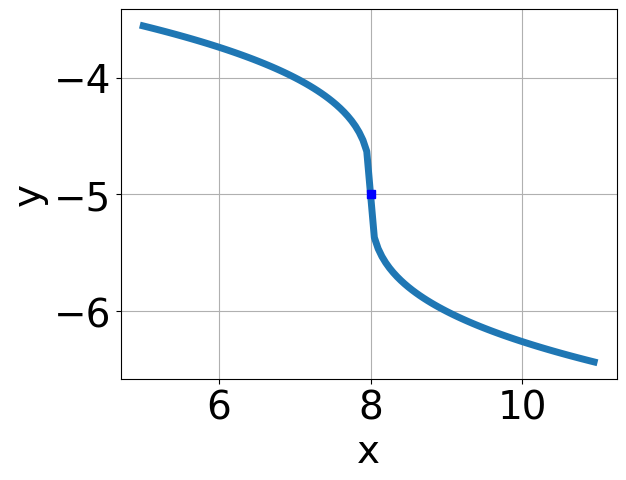
\includegraphics[width = 0.3\textwidth]{../Figures/radicalEquationToGraphBC.png}\item 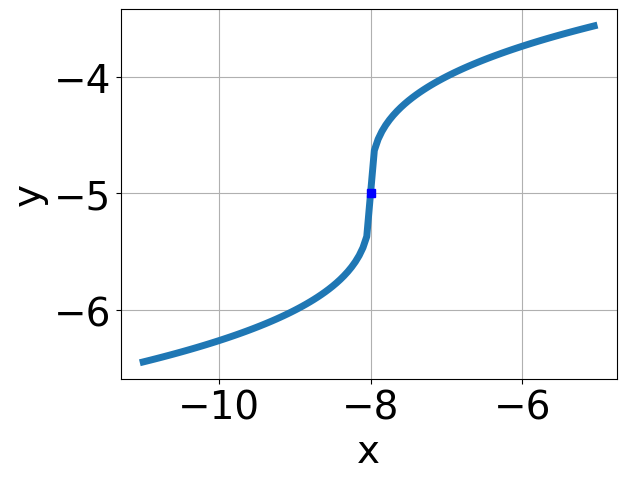
\includegraphics[width = 0.3\textwidth]{../Figures/radicalEquationToGraphCC.png}\item 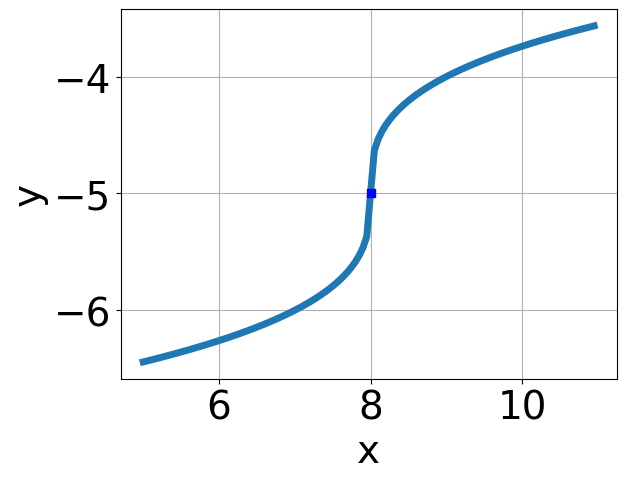
\includegraphics[width = 0.3\textwidth]{../Figures/radicalEquationToGraphDC.png}\end{multicols}\item None of the above.
\end{enumerate} }
\litem{
Solve the radical equation below. Then, choose the interval(s) that the solution(s) belongs to.\[ \sqrt{-18 x^2 + 54} - \sqrt{-69 x} = 0 \]\begin{enumerate}[label=\Alph*.]
\item \( x \in [2,6.3] \)
\item \( x_1 \in [0.6, 0.9] \text{ and } x_2 \in [1.5,7.5] \)
\item \( x \in [-2.5,0.2] \)
\item \( \text{All solutions lead to invalid or complex values in the equation.} \)
\item \( x_1 \in [-2.5, 0.2] \text{ and } x_2 \in [1.5,7.5] \)

\end{enumerate} }
\litem{
Solve the radical equation below. Then, choose the interval(s) that the solution(s) belongs to.\[ \sqrt{2 x - 7} - \sqrt{-4 x - 9} = 0 \]\begin{enumerate}[label=\Alph*.]
\item \( x \in [-1.8,-0.3] \)
\item \( x \in [2.3,3.4] \)
\item \( x_1 \in [-2.9, -1.2] \text{ and } x_2 \in [0.5,5.5] \)
\item \( x_1 \in [-1.8, -0.3] \text{ and } x_2 \in [0.5,5.5] \)
\item \( \text{All solutions lead to invalid or complex values in the equation.} \)

\end{enumerate} }
\litem{
Choose the equation of the function graphed below.
\begin{center}
    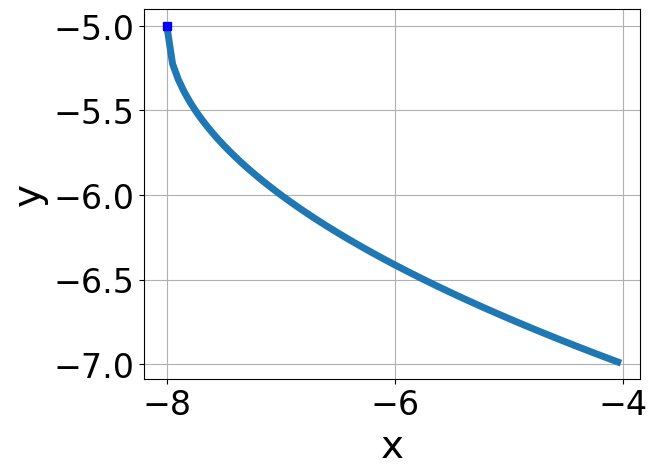
\includegraphics[width=0.5\textwidth]{../Figures/radicalGraphToEquationC.png}
\end{center}
\begin{enumerate}[label=\Alph*.]
\item \( f(x) = - \sqrt[3]{x - 8} - 5 \)
\item \( f(x) = \sqrt[3]{x - 8} - 5 \)
\item \( f(x) = \sqrt[3]{x + 8} - 5 \)
\item \( f(x) = - \sqrt[3]{x + 8} - 5 \)
\item \( \text{None of the above} \)

\end{enumerate} }
\litem{
What is the domain of the function below?\[ f(x) = \sqrt[8]{6 x - 4} \]\begin{enumerate}[label=\Alph*.]
\item \( (-\infty, \infty) \)
\item \( (-\infty, a], \text{where } a \in [0.9, 2.13] \)
\item \( (-\infty, a], \text{where } a \in [0.33, 0.73] \)
\item \( [a, \infty), \text{ where } a \in [0.22, 0.71] \)
\item \( [a, \infty), \text{where } a \in [1.48, 1.57] \)

\end{enumerate} }
\litem{
Choose the equation of the function graphed below.
\begin{center}
    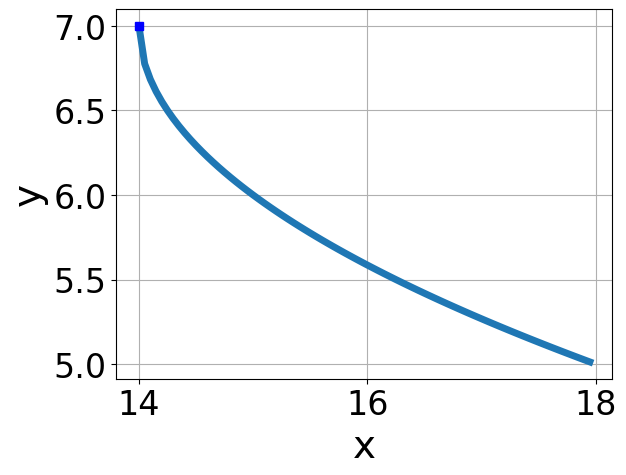
\includegraphics[width=0.5\textwidth]{../Figures/radicalGraphToEquationCopyC.png}
\end{center}
\begin{enumerate}[label=\Alph*.]
\item \( f(x) = - \sqrt[3]{x - 14} + 7 \)
\item \( f(x) = \sqrt[3]{x + 14} + 7 \)
\item \( f(x) = \sqrt[3]{x - 14} + 7 \)
\item \( f(x) = - \sqrt[3]{x + 14} + 7 \)
\item \( \text{None of the above} \)

\end{enumerate} }
\litem{
What is the domain of the function below?\[ f(x) = \sqrt[8]{-5 x - 3} \]\begin{enumerate}[label=\Alph*.]
\item \( [a, \infty), \text{where } a \in [-5.2, -1.5] \)
\item \( (-\infty, a], \text{where } a \in [-2.31, -1.53] \)
\item \( (-\infty, a], \text{ where } a \in [-0.64, -0.23] \)
\item \( (-\infty, \infty) \)
\item \( [a, \infty), \text{where } a \in [-0.7, 0.7] \)

\end{enumerate} }
\litem{
Solve the radical equation below. Then, choose the interval(s) that the solution(s) belongs to.\[ \sqrt{64 x^2 + 18} - \sqrt{88 x} = 0 \]\begin{enumerate}[label=\Alph*.]
\item \( x \in [0.33,2.19] \)
\item \( x_1 \in [-1.57, -0.3] \text{ and } x_2 \in [-3,0.3] \)
\item \( \text{All solutions lead to invalid or complex values in the equation.} \)
\item \( x \in [-0.97,1.04] \)
\item \( x_1 \in [-0.97, 1.04] \text{ and } x_2 \in [1.1,3.9] \)

\end{enumerate} }
\litem{
Solve the radical equation below. Then, choose the interval(s) that the solution(s) belongs to.\[ \sqrt{-5 x - 3} - \sqrt{-4 x - 7} = 0 \]\begin{enumerate}[label=\Alph*.]
\item \( x_1 \in [-2.81, -1.57] \text{ and } x_2 \in [-3.6,0.4] \)
\item \( x_1 \in [-1.07, -0.56] \text{ and } x_2 \in [4,5] \)
\item \( x \in [3.35,4.65] \)
\item \( \text{All solutions lead to invalid or complex values in the equation.} \)
\item \( x \in [-10.77,-8.12] \)

\end{enumerate} }
\end{enumerate}

\end{document}